\chapter{Background}


\section{Information Flow Analysis for JavaScript}

Information flow generally refers to the transfer of information from one variable x to the another variable y in a certain process. 
This chapter expands more on how to track information flow. Information flow control secures information mainly by limiting how exactly the information is communicated among the objects and users with various security classes. The main approach that is followed to keep track of this information flow is to label and track sensitive information. We associate each value within this JavaScript interpreter with a security label. These labels are the security classes dictating how a value may be used. 

These dynamic labels are needed to securely control information flow, especially when the access rights are changed dynamically and checked at runtime. Using these labels, the interpreter should never leak any secret to public users. 

\subsection{Explicit Flows}
Some times direct assignment leads to explicit flows as in 
\begin{figure}[h]
  \centering
\begin{lstlisting}[language=JavaScript, frame=none, numbers=none] 
 var l = h;
\end{lstlisting}
\end{figure}
here, as the value depends on the value of h, the system monitor labels l as secret as well.

This system updates the labels based on the labels of those values that influence the final result. For an addition operation the label of the result is decided by the join of other operand's labels. modifying an object's structure or that of an array by introducing or removing properties updates the label of that particular object to current context. Such changes can be observed by an attacker easily. 

\subsection{Implicit Flows}
Implicit flows arise through the program's control flow. 
\begin{figure}[h]
  \centering
\begin{lstlisting}[language=JavaScript, frame=none, numbers=none] 
 var l = 0;
 if (h) 
   l = 1;
\end{lstlisting}
\end{figure}
Given such a situation as above, the value of l depends on the value of h. Thus to handle such kind of implicit flows a new security label associated with the control flow has been introduced and is called the program counter (pc). The pc reflects the securing against the modification of less confidential data when the execution is influenced by confidential data.

Many previous papers on information flow control have only talked about languages without unstructured control flow. But many of the languages do have control statements such as break, continue, try ... catch ... finally. The implicit flows that come up with such kind of control flows are never to be ignored. In this paper I have worked on presenting an experimental way to deal with such kind of implicit flows.

Concentrating on dynamic mechanisms alone will not be helpful as they acquire excessive run-time overhead and might not prevent implicit flows that arising from the control flow paths that are not taken or observed during runtime. Thus, both dynamic labels and static information flow controls are combined to get the desired security. 

\subsection{Other existing information flow analysis}
\subsubsection{Secure Multi execution}
Secure multi execution (SME)  is a classic way to provide security by completing/running a program multiple times, once for every security level. It ensures for every executing level, the output produced is confined only to that security level and is dependent only on the input given to that level. Secure multiexecution guarantees non-interference ~\cite{multiproc1} ~\cite{secureMulti}. 

Static analysis accepts or rejects a particular program before it is run and there is no check performed once the program is started. In contrast to this, dynamic analysis makes some checks at runtime. Dynamic analysis seems more permissive, but on the other hand it will treat the paths/views that are not considered during the current execution in a more moderate way and might limits any change ~\cite{secureMulti}. 

Within secure multi-execution, security is achieved by separating the computations that are having different security principles. The program is executed as many times as there are number of security levels within the program and different outputs are seen in a different way for obvious reasons.

Consider the following JavaScript code used to send an email.

\begin{figure}[h]
  \centering
\begin{lstlisting}[language=JavaScript] 
	var text = document.getElementById('email-input').text;
	var abc = 0;
	if(text.indexOf('abc')!=-1) { 
		abc = 1 
	};
	var url = 'http://example.com/img.jpg?t=' + escape(text) + abc;
	document.getElementById('banner-img').src = url;
\end{lstlisting}
\caption[Information Flow]
    {}
    \label{fig:SME1}
\end{figure}

The expression "{\it document.getElementById('email-input').text}" could be considered as an input at security level H (confidential). The expression "{\it document.getElementById('banner-img').src}" could be considered as an output at security level L (public). The example in Figure ~\ref{fig:SME1} displays an information flow from a high level input(H) into a low level output (L). In this classification, this unacceptable flow can be eliminated by a property called \textbf{non-interference}. 

\subsubsection{Non-Interference}
The goal here is to avert attackers from gaining access to any kind of information that is confidential. In other words, if a program has same level of inputs, lets say public, for two parallel executions, then it must produce the same level of outputs no matter how confidential the inputs are.

A system is said to have \textbf{non-interference} property if and only if there is no dependency on the high level input and it produces the same low level outputs for any corresponding low level inputs. That is, a low level user will never be able to gain any information on the activities of a high level user. Non-interference has two different types. \\
1) Termination-sensitive\\
2) Termination-insensitive

Termination-sensitive non-interference makes sure that no information is lost due to termination behavior of the program. Termination-insensitive non-interference (TINI) leaks only a single bit of information  and that is due to the program's termination behavior.

Now consider the following program with different levels of execution.

\begin{figure}[h]
  \centering
\begin{lstlisting}[language=JavaScript] 
var text = undefined; 
var abc = 0; 
if(text.indexOf('abc')!=-1) { 
	abc = 1 
}; 
var url = 'http://example.com/img.jpg?t=' + escape(text) + abc;
document.getElementById('banner-img').src = url;
\end{lstlisting}
\caption[Execution at L security level.]
    {Execution at L security level. Multi-Execution of JavaScript program from Figure ~\ref{fig:SME1}}
    \label{fig:SME2}
\end{figure}

\begin{figure}[h]
  \centering
\begin{lstlisting}[language=JavaScript] 
var text = document.getElementById('email-input').text; 
var abc = 0; 
if(text.indexOf('abc')!=-1) { abc = 1 }; 
var url = 'http://example.com/img.jpg?t=' + escape(text) + abc;
\end{lstlisting}
\caption[Execution at H security level.]
    {Execution at H security level. Multi-Execution of JavaScript program from Figure ~\ref{fig:SME1}}
    \label{fig:SME3}
\end{figure}


\section{Faceted Evaluation Overview}
We have seen the problems caused by implicit flows. To overcome that, the Faceted Value approach has been put forward in the previous papers ~\cite{bib3} ~\cite{bib4}. Consider the following example where
\begin{figure}[h]
  \centering
\begin{lstlisting}[language=JavaScript, frame=none, numbers=none] 
 var l = 0 ;
  if (h) 
    l = 1;
\end{lstlisting}
\end{figure}
the value of l depends on the authority of the observer. if {\it h } is secret here, then  \par 
	-a private observer who has access to {\it h } reads {\it l } as 1; \par
	-a public observer who doesn't have access to {\it h } reads it as 0;\par
\noindent Looking at this, A faceted value can be explained as a triple that consists of a principle k and then followed by two values $V_{H}$ and $V_{L}$. Faceted values showcase the dual nature of l that has to be 0 or 1 based on the user\textquotesingle s authority. Below is how a faceted value can be written
$$
 <k\ ?\ V_{H}\ :\ V_{L}>
$$
A private observer can see $V_{H}$ and public observer can see $V_{L}$. But if there is a need to represent a single value V where it needs to be private, it can be showcased as
$$
 <k\ ?\ V\ :\ \bot>
$$
A faceted value can be nested. Consider the example below. 
$$
 <k_{1}\ ?\ true	\ :\ \bot> \&\& <k_{2}\ ?\ false\ :\ \bot>
$$
The above expression can be evaluated to 
$$
 <k_{1}\ ?\ <k_{2}\ ?\ false\ :\ \bot>\ :\ \bot>
$$
where $k_{1}$ and $k_{2}$ are two different principals.

\begin{figure}
\centering
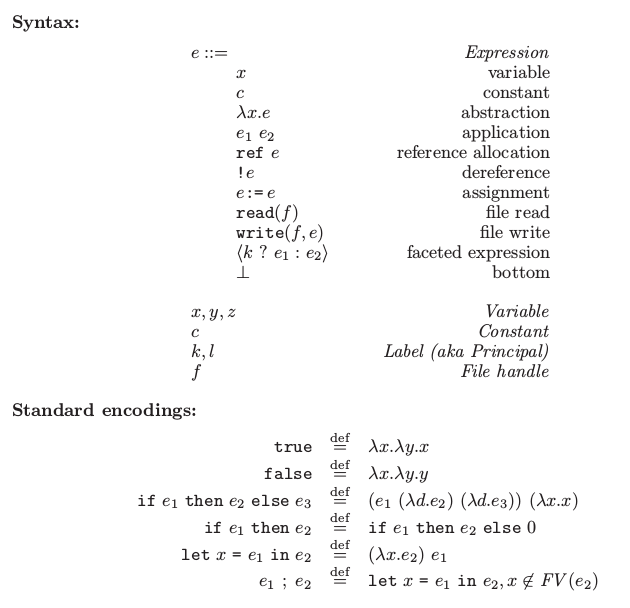
\includegraphics[width=1\textwidth]{images/LambdaFacet.png}
\caption[The source language $\lambda_{facet}$.]{The source language $\lambda_{facet}$. \\ Source: ~\cite{bib4} } 
\label{fig:Source_Language}
\end{figure}

Using these Faceted Values, a previous paper ~\cite{bib3} developed a dynamic analysis that exactly tracks information flow. If a control flow comes across a faceted value as shown in Figure ~\ref{fig:facetEvalCF},
\begin{figure}[h]
  \centering
\begin{lstlisting}[language=JavaScript] 
 var k = <$k_{1}$ ? 0 : 1>;
 if (k) 
   e1; 
 else e2;
\end{lstlisting}
\caption[Faceted evaluation - control flow.]
    {Faceted evaluation - control flow.}
    \label{fig:facetEvalCF}
\end{figure}
both $e_{1}$ and $e_{2}$ are executed carefully and whatever evaluations or assignments that are performed during the $e_{1}$ phase are only observed by private users and those of $e_{2}$ by public users. After both the evaluations are completed, the results are combined into a single faceted value and the flow continues. We can have a closer look at the examples in later chapters.

\subsection{Exceptions Overview}

Handling exceptions with faceted values introduces many challenges. An exception raised in a single view should not influence the other view especially when the exception is raised in a higher level view. Intruders can have a chance to send out few values that might raise an exception and thus try to get a handle on the actual information by repeatedly sending such kind if information. These implicit flows needs to be properly handled. Consider the example Figure ~\ref{fig:facetExcepCF}
\begin{figure}[h]
  \centering
\begin{lstlisting}[language=JavaScript] 
 function parseJSON( jsonStr) {
      var obj = {};
      try {
           eval (" obj = " + jsonStr);
      } catch (e) {
          console.log(e);
          throw e;
      }
      return obj;
 }
\end{lstlisting}
\caption[Faceted exception - control flow.]
    {Faceted exception - control flow. \\ This function accepts a JSON string as an input and assigns it to an object obj. If the given JSON string is malformed an exception is thrown at line 4.}
    \label{fig:facetExcepCF}
\end{figure}

if the parameter jsonStr that is sent to this function in Figure ~\ref{fig:facetExcepCF} is of this form,
$$
 <k\ ?\ ``\{name:`smith', balance:2543''\ :\ ``\{\ \}''>  
$$
then for a higher level view there will be a syntax error thrown. But we need to make sure that does not affect what a lower level user can see and this exception should not be visible in that view. In this paper, I will be presenting a proper way to handle this kind of exception and make sure the control flow is proper and the program does not crash.


The main theme about Faceted Evaluation is to mimic the multiple executions of SME. Labelled approach in many situations, lacks certain important features. This paper reviews the semantics of faceted values with exceptions for minimal language $\lambda_{facet}$ and provides implementation for JavaScript using Narcissus ~\cite{kuno} and Zaphod ~\cite{Zaphod} libraries. 

\begin{figure}
\centering
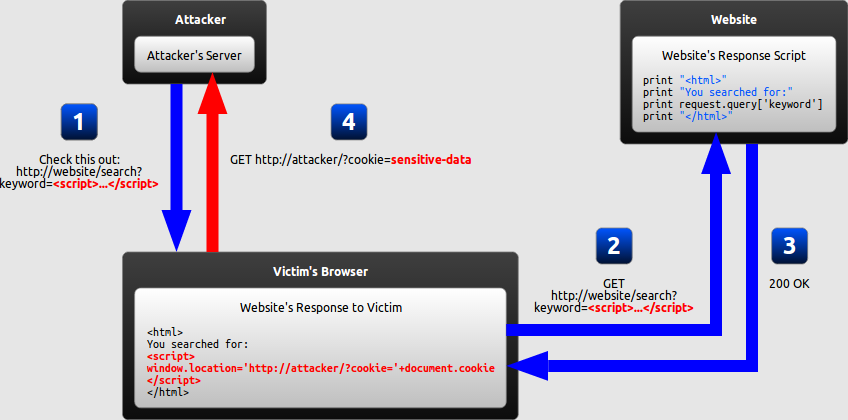
\includegraphics[width=1\textwidth]{images/reflected-xss.png}
\caption[Reflected XSS]{Reflected XSS. \\Source: ~\cite{attacks} } 
\label{fig:reflectedXSS}
\end{figure} 

\section{JavaScript Attacks}
JavaScript and the Document Object Model are the main source of security attacks. They provide a way for malicious users to inject third party scripts and allowing them to run on the client computer via the webpage. A common security problem related to JavaScript is cross-site scripting or XSS, which is a violation of the same-origin policy. 

The main goal of the attacker to implement XSS attack is to introduce the malicious script into the webpage of the victim. This script appears to be from the same site that is being attacked and thus user's browser cannot identify the script being executed is a part of the same site that the they are viewing ~\cite{XSS}. This can be achieved by submitting some special values through webforms. Figures ~\ref{fig:DOMXSS1}, ~\ref{fig:DOMXSS2} shows few examples of JavaScript attacks.

\begin{figure}
\centering
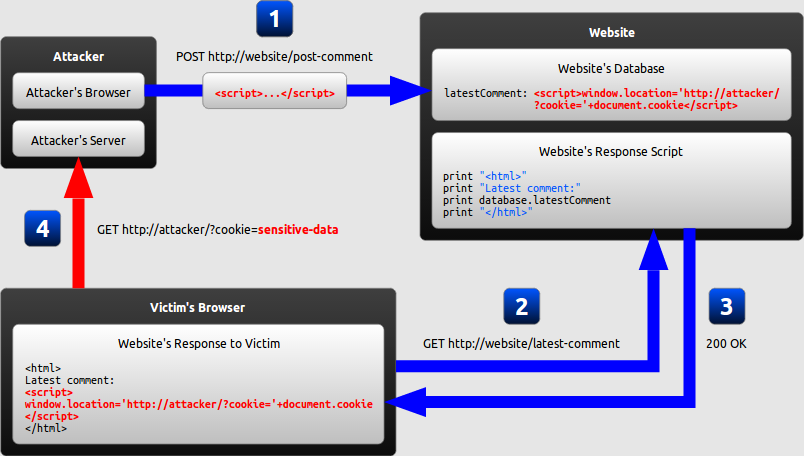
\includegraphics[width=1\textwidth]{images/persistent-xss.png}
\caption[Persistent XSS]{Persistent XSS. \\Source: ~\cite{attacks} } 
\label{fig:PersistentXSS}
\end{figure}

\begin{figure}[h]
  \centering
\begin{lstlisting}[language=JavaScript] 
 <SCRIPT>
var output=document.URL.indexOf("parameter=")+10;
document.write(document.URL.substring(output,document.URL.length));
</SCRIPT>
\end{lstlisting}
\caption[DOM based XSS attack 1]
    {Script to write on the screen from a url parameter. This can be used to gain access to user's session cookie by sending a url as shown in Figure ~\ref{fig:DOMXSS2}}
    \label{fig:DOMXSS1}
\end{figure}


\begin{figure}[h]
  \centering
\begin{lstlisting}[language=JavaScript] 
www.mysite.com/page.html?parameter=<script>alert(document.cookie)</script>
\end{lstlisting}
\caption[DOM based XSS attack 2]
    {URL used to attack.}
    \label{fig:DOMXSS2}
\end{figure}

\subsection{Different types of XSS attacks}
Persistent XSS, malicious string is a part of website's database. Figure ~\ref{fig:PersistentXSS}

Reflected XSS, malicious string will be a part of the victim's request. Figure ~\ref{fig:reflectedXSS}

DOM-based XSS, vulnerability is seen within the client-side code. Figures ~\ref{fig:DOMXSS1}, ~\ref{fig:DOMXSS2} shows DOM based attack.

\subsection{Clickjacking}
Advertising is the source of numerous incidents involving malicious JavaScript code. Attacker tries to intercept any click that user clicks on the advertise and makes the browser to redirect to thirdparty site by populating the URL to document.location ~\cite{jsattackclick}.
\begin{figure}[h]
  \centering
\begin{lstlisting}[language=JavaScript] 
document.addEventListener("click",new function() {
	document.location = "http://www.evil.com";
});
\end{lstlisting}
\caption[DOM based XSS attack 2]
    {URL used to attack.}
    \label{fig:clickjackingattack}
\end{figure}
Once, the user is redirected, then the site may install malware onto the user's system. Details on this attack are available on Google Caja's website ~\cite{caja}

In order to prevent this kind of attack, we generally restrict write to document.location to all the scripts hosted on the trusted/current site. All other scripts that are loaded from the other domains are marked as untrusted. DOM objects are updated as untrusted facets for simple usage except the DOM objects like document.location, which is treated as high-integrity. Usage of faceted values helps us in using the authorized/trusted facet if the URL is a faceted value. Thus by marking the code from external sites as untrusted and limiting its ability to update critical fields, we achieve key integrity properties.

